\documentclass[english,11pt,a4paper,titlepage]{article}

\usepackage{fontspec} % !!!Requires compiling with either XeLaTeX or LuaLaTeX!!! - allows for advanced font selection - also handles font encoding. If you wish to use PDFLaTeX with a natively supported font, you can use the following package instead:
% \usepackage[T1]{fontenc} 

\usepackage{amsmath} % Package for math notation
\usepackage{fontspec} % Requires either XeLaTeX or LuaLaTeX
\usepackage{titlesec} % Allows alternative section titles
\usepackage{lastpage} % Used for "n of m" page numbering
\usepackage{afterpage} % Used to remove background color from pages after title page
\usepackage{amsmath} % Package for math notation
\usepackage{setspace}% Package for easy line spacing 
\usepackage{titlesec} % Allows alternative section titles
\usepackage{lastpage} % Used for "n of m" page numbering
\usepackage{afterpage} % Used to remove custom page color of the front page from the remaining pages
\usepackage{microtype} % Improves spacing between words and letters
\usepackage{abstract} % Custom abstract section
\usepackage{setspace} % Package for easy line spacing 
\usepackage{xcolor} % Kind of self-explanatory... Handles colors
\usepackage{graphicx} % Handling graphics
\usepackage{fancyhdr} % Increased control over headers and footers
\usepackage{caption}

% ------Package suggestions------
\usepackage[backend=biber, style=numeric-comp, sorting=none]{biblatex} % Management of bibliography
% \usepackage{cleveref} % Enhanced cross-referencing of sections, figures, equations, etc.
\usepackage{booktabs} % For better looking tables - highly recommended!
% \usepackage{siunitx} % Useful for typesetting units and numbers
\usepackage{hyperref} % Enables hyperlinks within the LaTeX document and can make ToC, references, and more clickable
% \usepackage{listings} % Useful for writing algorithms / pseudocode
% \usepackage{mhchem} % Typesetting of chemical formulas and reactions
% ------------------------------

% Bibliography
\addbibresource{references.bib}

% Custom colours
\definecolor{sectioncolor}{RGB}{0,61,115} % Dark blue color 
\definecolor{subsectioncolor}{RGB}{75,75,74} % Grey color

% Heading font
\newfontfamily\headingfont{AUPassata_RG} % Standard AU font, replace this with your favourite font if needed

\titleformat*{\section}{\LARGE\headingfont\color{sectioncolor}}
\titleformat*{\subsection}{\Large\headingfont\color{subsectioncolor}}

% Configure the header
\pagestyle{fancy}
\fancyhf{} % Clears all header and footer fields
%\fancyhead[L]{
\includegraphics[height=1.1cm]{img/au_blue2.png}} % No department
%\fancyhead[L]{
\includegraphics[height=1.5cm]{img/inano.png}} % Interdisciplinary Nanoscience department
%\fancyhead[L]{
\includegraphics[height=1.5cm]{img/mbg.png}} % Molecular Biology department
\fancyhead[L]{
\includegraphics[height=1.5cm]{img/birc.png}} % Bioinformatics Research department

\fancyhead[R]{
\includegraphics[height=1.5cm]{img/ausegl.png}} % Dolphin seal

\fancyfoot[C]{\headingfont\thepage} % Page number in footer
%\fancyfoot[C]{\headingfont\thepage\ of \pageref{LastPage}} % "m of n" page numbering in footer


\usepackage{geometry} % Allows easy change of page layout (margin size etc.)
% Page layout
\geometry{
	top=0.5cm, % Adjust top margin
	right=4.2cm, % Adjust right margin
	left=4.2cm, % Adjust left margin,
	bottom=3cm, % Adjust bottom margin
	headheight=3.5cm, % Adjust header height
	headsep=1.0cm, % Spacing between header and text
	includeheadfoot % Include header and footer
	}

% Main font
\setmainfont{Georgia}




\usepackage{kantlipsum} % Sample text - can be removed 




\newfontfamily\titlefont{AUPassata_BOLD} % Font for paper title

% ------------------------------ Custom Front Page Commands ------------------------------
% These commands define the layout and styling for the front pages of the document.
% They require 7 parameters:
% #1: The title of the document.
% #2: The first author's name.
% #3: The department or affiliation of the first author.
% #4: The second author's name (if applicable).
% #5: The department or affiliation of the second author (if applicable).
% #6: Path to an image file to be displayed on the front page.
% #7: Any additional information or text to be included at the bottom (e.g., supervisor's name).
% Example usage: \frontpageBlue{My Title}{My Name}{My Department}{Partner's Name}{Partner's Department}{path/to/image.jpg}{Additional Info}


% Setup for front page with blue background color
\newcommand{\frontpageBlue}[8]{
	\begin{titlepage}
		\pagecolor{sectioncolor}\afterpage{\nopagecolor}
		\centering
		\includegraphics[width=0.5\textwidth]{#7}\par
		\vspace{1cm}
		{\fontsize{34}{40}\selectfont\color{white}\titlefont #1\par} % Title
		\vspace{2cm}
		{\color{white}\Large\headingfont #2\par} % Author 1
		{\color{white}\large\headingfont #3\par} % Department author 1
		\vspace{1cm}
		{\color{white}\Large\headingfont #4\par} % Author 2
		{\color{white}\large\headingfont #5\par} % Department author 2
		\vspace{1cm}
		\includegraphics[width=0.5\textwidth]{#8} % Image
		\vfill
		%{\color{white}\Large\headingfont Supervisor\par} % Additional info
		{\color{white}\Large\headingfont #6}
	\end{titlepage}
}


% Setup for front page with white background color
\newcommand{\frontpageWhite}[8]{
	\begin{titlepage}
		\centering
		\includegraphics[width=0.5\textwidth]{#7}\par
		\vspace{1cm}
		{\fontsize{26}{28}\selectfont\color{sectioncolor}\titlefont #1\par} % Title
		\vspace{2cm}
		{\Large\headingfont\color{sectioncolor} #2\par} % Author 1
		{\large\headingfont\color{sectioncolor} #3\par} % Department author 1
		\vspace{0.1cm}
		{\Large\headingfont\color{sectioncolor} #4\par} % Author 2
		{\large\headingfont\color{sectioncolor} #5\par} % Department author 2
		\vspace{1cm}
		\includegraphics[width=0.5\textwidth]{#8} % Image
		\vfill
		%{\Large\headingfont\color{sectioncolor} Supervisor\par} % Additional information
		{\Large\headingfont\color{sectioncolor} #6}
	\end{titlepage}	
}

% Setting up the abstract section
\renewcommand{\abstractnamefont}{\normalfont\Large\bfseries} % Set the "Abstract" title to bold
\renewcommand{\abstracttextfont}{\normalfont\small\itshape} % Set the abstract itself to italic



%-----------------Beginning of document--------------------


\begin{document}
\setstretch{1.309} % Line spacing
\setlength{\parindent}{25pt} % Indentation at beginning of new paragraph


% ------ Blue front page ------
%\frontpageBlue{A systematic review of...}{Sample Author One}{Sample Department One}{Sample Author Two}{Sample Department Two}{}{img/ausegl_hvid.png}{img/au_white.png}


% ------ White front page ------
\frontpageWhite{Enhancing Antimicrobial Resistance Prediction with Convolutional Neural Networks}{Rasmus Freund}{Bioinformatics Research Center}{}{}{Supervisor\\Palle Villesen}{img/ausegl.png}{img/au_blue.png}


\begin{abstract}
	\noindent % No indentation for abstracts!
	\kant[1]
\end{abstract}

\captionsetup{font=small}

\section*{Introduction}
Antimicrobial resistance (AMR) presents one of the most daunting challenges in global public health, threatening to render ineffective the very drugs designed to protect us from bacterial infections. The pervasiveness and impact of AMR are profound, as bacteria continue to evolve mechanisms to survive against antibiotics, which have historically revolutionized the management of infectious diseases. 

In 2019, an estimated 4.95 million deaths were associated with bacterial AMR, with 1.27 million directly attributable to drug resistance	\cite{murrayGlobalBurdenBacterial2022}. The predominant pathogens contributing to AMR-related deaths include \textit{Eschericia coli}, \textit{Staphylococcus aureus}, and \textit{Klebsiella pneumoniae}, among others, which are responsible for a significant proportion of the mortality associated with drug-resistant infections. These bacteria are particularly dangerous due to their ability to resist multiple drugs, which complicates treatment options and increases the risk of severe outcomes \cite{murrayGlobalBurdenBacterial2022}.

Given the critical need for rapid and accurate antimicrobial resistance testing, this thesis explores advanced machine learning approaches to predict AMR directly from MALDI-TOF mass spectra of clinical isolates. Central to this work is the use of the Database of Resistance Information on Antimicrobials and MALDI-TOF Mass Spectra (DRIAMS), a comprehensive and publicly available dataset created by a collaborative effort of researchers from ETH Zürich, the University of Basel, and other institutions \cite{weis2021driams}.

From 2016 to 2018, DRIAMS compiled over 300,000 mass spectra and more than 750,000 antimicrobial resistance phenotypes from clinical isolates collected across four diagnostic laboratories in Switzerland. This extensive dataset encompasses 803 different species of bacterial and fungal pathogens and is organized into four subcollections (DRIAMS-A to DRIAMS-D) \cite{weisDirectAntimicrobialResistance2022}. DRIAMS-A, the largest subcollection, serves as the primary focus of this thesis and contains 145,341 mass spectra linked to 71 different antimicrobial drugs.

To address the challenges posed by AMR, this thesis adopts a multi-stage approach, starting with the application of standard machine learning models to predict bacterial species from MALDI-TOF spectra. Building on this foundation, the focus then shifts to predicting AMR using a variety of machine learning techniques. As the complexity of the problem increases, more advanced techniques are employed to better capture the intricate patterns in the data and potentially enhance prediction accuracy and reliability. The following sections will explore these techniques in detail.


	\subsection*{Understanding Machine Learning}
	Machine learning (ML) is a subfield of artificial intelligence (AI) focused on developing algorithms that allow computers to learn from and make predictions or decisions based on data. Unlike traditional programming, where specific instructions are coded by humans, ML systems improve their performance on tasks through experience.
	
	The essence of ML lies in its ability to identify patterns and relationships with large datasets, which might be too complex or subtle for humans to discern. This capability is particularly valuable in fields like bioinformatics, where the volume and complexity of data, such as those found in genomic sequences or mass spectra, require advanced analytical methods.
	
	\subsubsection*{Basic Concepts of Machine Learning}
	At its core, ML can be divided into three main types: supervised learning, unsupervised learning, and reinforcement learning.
	\begin{itemize}
		\item \textbf{Supervised Learning}: In supervised learning, the algorithm is trained on a labeled dataset, meaning that each training example is paired with an output label. The goal is to learn a mapping from inputs to outputs that can be used to predict the labels of new, unseen examples. Common algorithms include linear regression, decision trees, and neural networks \cite{jordanMachineLearningTrends2015}.
		\item \textbf{Unsupervised Learning}: Unsupervised learning deals with unlabeled data. The algorithm tries to learn the underlying structure of the data without explicit instructions on what to predict. Techniques like clustering and dimensionality reduction fall under this category. Probabilistic models, such as Gaussian Mixture Models (GMM) and algorithms like k-means and with principal component analysis (PCA), are often used to uncover hidden patterns in the data \cite{ghahramaniProbabilisticMachineLearning2015}.
		\item \textbf{Reinforcement Learning}: In reinforcement learning, an agent learns to make decisions by performing actions in an environment to maximize cumulative reward. The agent, which can be a software program or a robot, interacts with the environment by taking actions and receiving feedback in the form of rewards or penalties. This feedback helps the agent learn the optimal strategy to achieve its goals over time \cite{suttonReinforcementLearningIntroduction}. While reinforcement learning represents a significant area of ML research, it is not utilized in this thesis. Its mention here serves to provide a comprehensive overview of the main types of machine learning.
	\end{itemize}
	
	\subsection*{Regularized Linear Regression: Ridge and LASSO}
	Regularized linear regression techniques, such Ridge and LASSO (short for Least Absolute Shrinkage and Selection Operator), address overfitting by introducing a penalty term to the least squares objective function. Overfitting occurs when a model is too complex and captures noise in the training data, leading to poor generalization on unseen data. These methods are particularly useful in high-dimensional scenarios, where they can improve generalization and perform feature selection.
	
	\subsubsection*{Mathematical Formulation}
	In standard linear regression, the objective is to minimize the sum of squared residuals:
	\begin{equation*} 
		\min_\beta \sum_{i=1}^{n}(y_i - X_i\beta)^2
	\end{equation*}
	where $X$ is the matrix of input features, $y$ is the vector of target values, and $\beta$ is the vector of coefficients.
	
	Ridge Regression modifies the objective by adding a regularization term that penalizes large coefficients:
	\begin{equation*}
		\min_\beta \left[\sum_{i=1}^{n}(y_i - X_i\beta)^2 + \lambda \sum_{j=1}^{p}\beta_{j}^{2}\right]
	\end{equation*}
	Here, $\sum_{j=1}^{p}\beta_{j}^{2}$ represents the L2 norm (Euclidean norm) of the coefficients, which is the sum of the squared values of the coefficients. The L2 norm penalizes large coefficients, encouraging them to be small but not necessarily zero.
	
	LASSO Regression, on the other hand, adds a regularization term that penalizes the absolute values of the coefficients:
	\begin{equation*}
		\min_\beta \left[\sum_{i=1}^{n}(y_i - X_i\beta)^2 + \lambda \sum_{j=1}^{p}|\beta_{j}|\right]
	\end{equation*}
	Here, $\sum_{j=1}^{p}|\beta_{j}|$ represents the L1 norm (Manhattan norm) of the coefficients, which is the sum of the absolute values of the coefficients. The L1 norm can drive some coefficients to exactly zero, performing feature selection.
	
	Additionally, we can see that setting \( \lambda = 0 \) for either Ridge or LASSO reduces the respective expression to ordinary least squares (OLS) regression.
	
	\subsubsection*{Application to Classification}
	While Ridge and LASSO are primarily used for regression tasks, they can be adapted for classification through logistic regression \cite{friedmanRegularizationPathsGeneralized2010,hastieElementsStatisticalLearning2009}. Logistic regression uses the logistic function to model the probability that a given input point belongs to a specific class:
	\begin{equation*}
		P(y=1|X) = \frac{1}{1 + e^{-X\beta}}
	\end{equation*}
	To fit a logistic regression model, we maximize the likelihood of the observed data. The likelihood function measures the probability of the observed labels given the input data and model parameters \cite{whitlockAnalysisBiologicalData2015}. For binary classification, the likelihood of the data is given by:
	\begin{equation*}
		L(\beta) = \prod_{i=1}^{n} P(y_i | X_i)
	\end{equation*}
	Taking the natural logarithm of the likelihood function, we obtain the log-likelihood:
	\begin{equation*}
		\log L(\beta) = \sum_{i=1}^{n} \left[ y_i \log P(y=1|X_i) + (1-y_i) \log (1 - P(y=1|X_i)) \right]
	\end{equation*}
	Maximizing the log-likelihood is equivalent to minimizing the negative log-likelihood (NLL), which measures the discrepancy between the observed labels (\( y_i \)) and the predicted probabilities (\( P(y = 1 | X_i )\)):
	\begin{equation*}
		\text{NLL}(\beta) = -\sum_{i=1}^{n} \left[ y_i \log P(y=1|X_i) + (1-y_i) \log (1 - P(y=1|X_i)) \right]
	\end{equation*}
	To regularize logistic regression, the NLL is combined with a penalty term, as shown below.
	
	\noindent
	\textbf{Ridge Logistic Regression} \\
	Adds an L2 penalty term to the negative log-likelihood:
	\begin{equation*}
		\min_{\beta} \left[ -\sum_{i=1}^{n} \left( y_i \log P(y=1|X_i) + (1-y_i) \log (1 - P(y=1|X_i)) \right) + \lambda \sum_{j=1}^{p}\beta_{j}^{2} \right]
	\end{equation*}
	
	\noindent
	\textbf{LASSO Logistic Regression} \\
	Adds an L1 penalty term to the negative log-likelihood:
	\begin{equation*}
		\min_{\beta} \left[ -\sum_{i=1}^{n} \left( y_i \log P(y=1|X_i) + (1-y_i) \log (1 - P(y=1|X_i)) \right) + \lambda \sum_{j=1}^{p}|\beta_{j}| \right]
	\end{equation*}
	
	\subsubsection*{Properties and Benefits}
	\begin{itemize}
		\item \textbf{Bias-Variance Tradeoff}: Both Ridge and LASSO introduce bias by shrinking the coefficients, but this can reduce the model's variance and improve generalization performance \cite{sohilIntroductionStatisticalLearning2022} (see Figures \ref{fig:ridgelambdaeffect} and \ref{fig:lassolambdaeffect}).
		\item \textbf{Handling Multicollinearity (Ridge)}: Ridge Regression mitigates multicollinearity (high level of correlation between several input features) by shrinking coefficients, thus providing more stable estimates \cite{hoerlRidgeRegressionBiased1970,marquardtRidgeRegressionPractice1975}.
		\item \textbf{Feature Selection (LASSO)}: LASSO can shrink some coefficients to exactly zero, thus performing feature selection and simplifying the model. This is particularly beneficial in high-dimensional datasets \cite{tibshiraniRegressionShrinkageSelection1996}.
	\end{itemize}
	
	To effectively apply Ridge and LASSO regression, it is crucial to select the appropriate regularization parameter \( \lambda \) - cross-validation is a robust technique for determining an optimal value \cite{sohilIntroductionStatisticalLearning2022}. This process involves:
	\begin{enumerate}
		\item \textbf{Splitting the data}: Divide the dataset into \( k \) folds (e.g., \( k = 5 \) or \( k = 10 \))
		\item \textbf{Training and Validation}: Train the model on \( k - 1 \) folds and validate it on the remaining fold. This process is repeated \( k \) times, with each fold serving as the validation set once.
		\item \textbf{Averaging Performance}: Calculate the average performance metric (e.g., mean squared error) across all \( k \) folds for different values of \( \lambda \)
		\item \textbf{Selecting \( \lambda \)}: Choose the \( \lambda \) that minimizes the average validation error, ensuring the model generalizes well to unseen data
	\end{enumerate}
	
	\subsection*{Elastic Net Regression}
	Elastic Net Regression is a regularized regression technique that linearly combines the penalties of Ridge and LASSO. It is particularly useful when dealing with high-dimensional data where multicollinearity is present and when feature selection is necessary.
	
	\subsubsection*{Mathematical Formulation}
	Elastic Net modifies the objective of standard linear regression by adding two regularization terms:
	\begin{equation*}
		\min_\beta \left[\sum_{i=1}^{n}(y_i - X_i\beta)^2 + \lambda_1 \sum_{j=1}^{p}|\beta_{j}| + \lambda_2 \sum_{j=1}^{p}\beta_{j}^{2}\right]
	\end{equation*}
	Here, $\lambda_1$ controls the LASSO penalty (L1 norm) and $\lambda_2$ controls the Ridge penalty (L2 norm). When both $\lambda_1$ and $\lambda_2$ are zero, Elastic Net reduces to OLS regression. By adjusting these parameters, Elastic Net can balance between the benefits of Ridge and LASSO, shrinking some coefficients while performing feature selection \cite{zouRegularizationVariableSelection2005}.
	
	\begin{figure}[!t]
		\centering
		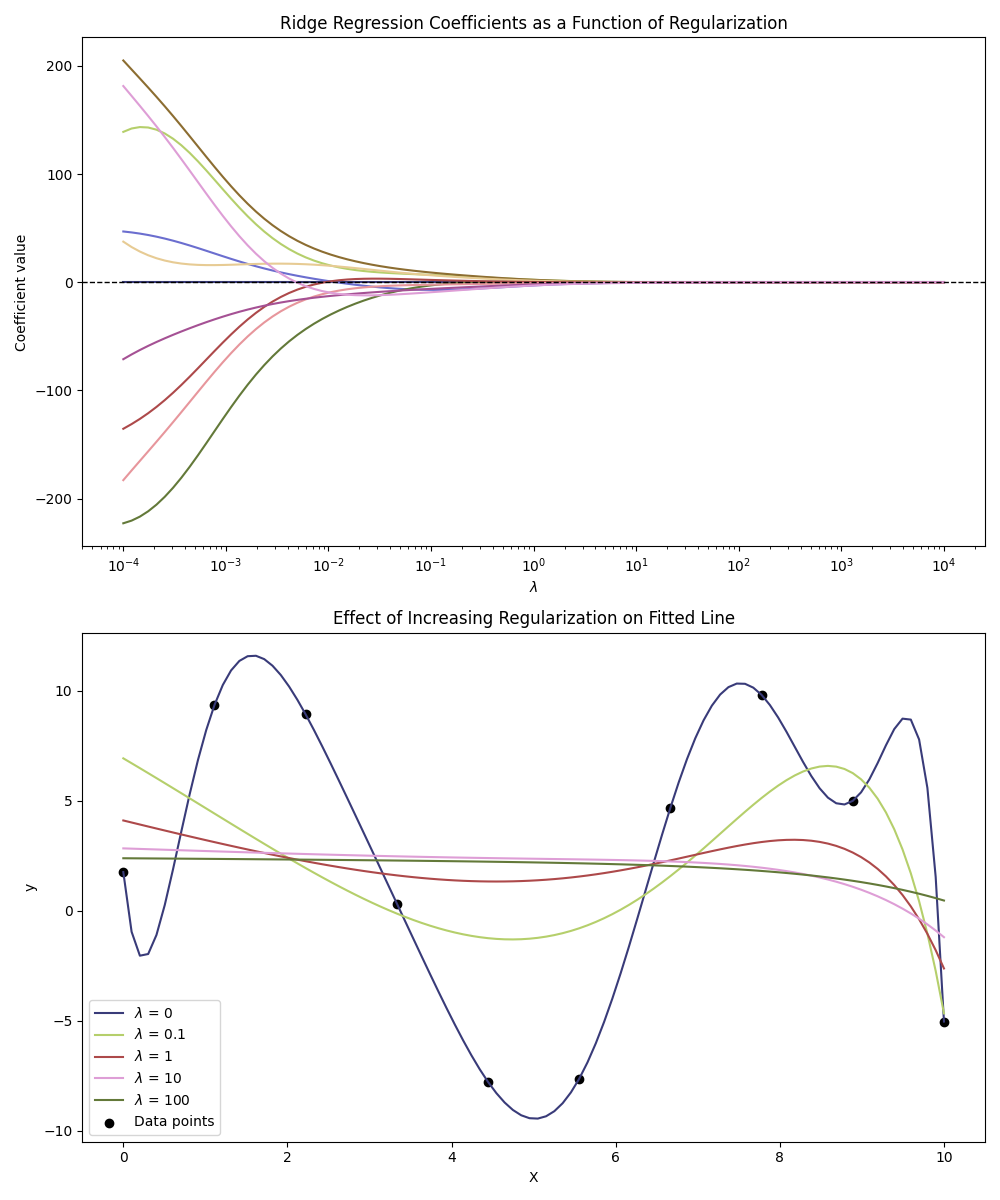
\includegraphics[width=1.0\linewidth]{img/ridge_lambda_effect}
		\caption{Ridge Regression Coefficients and the Effect of Regularization. \\ The \textbf{top plot} shows Ridge Regression coefficients as a function of the regularization parameter $\lambda$. Each line represents a different feature's coefficient, demonstrating how increasing $\lambda$ causes the coefficients to shrink towards zero. The \textbf{bottom plot} illustrates the effect of $\lambda$ on the fitted non-linear model for 10 data points (synthetic data). As $\lambda$ increases, the model transitions from overfitting (high variance) to better generalization (low variance), as seen by the smoothing of the fitted lines.}
		\label{fig:ridgelambdaeffect}
	\end{figure}
	
	\begin{figure}[!t]
		\centering
		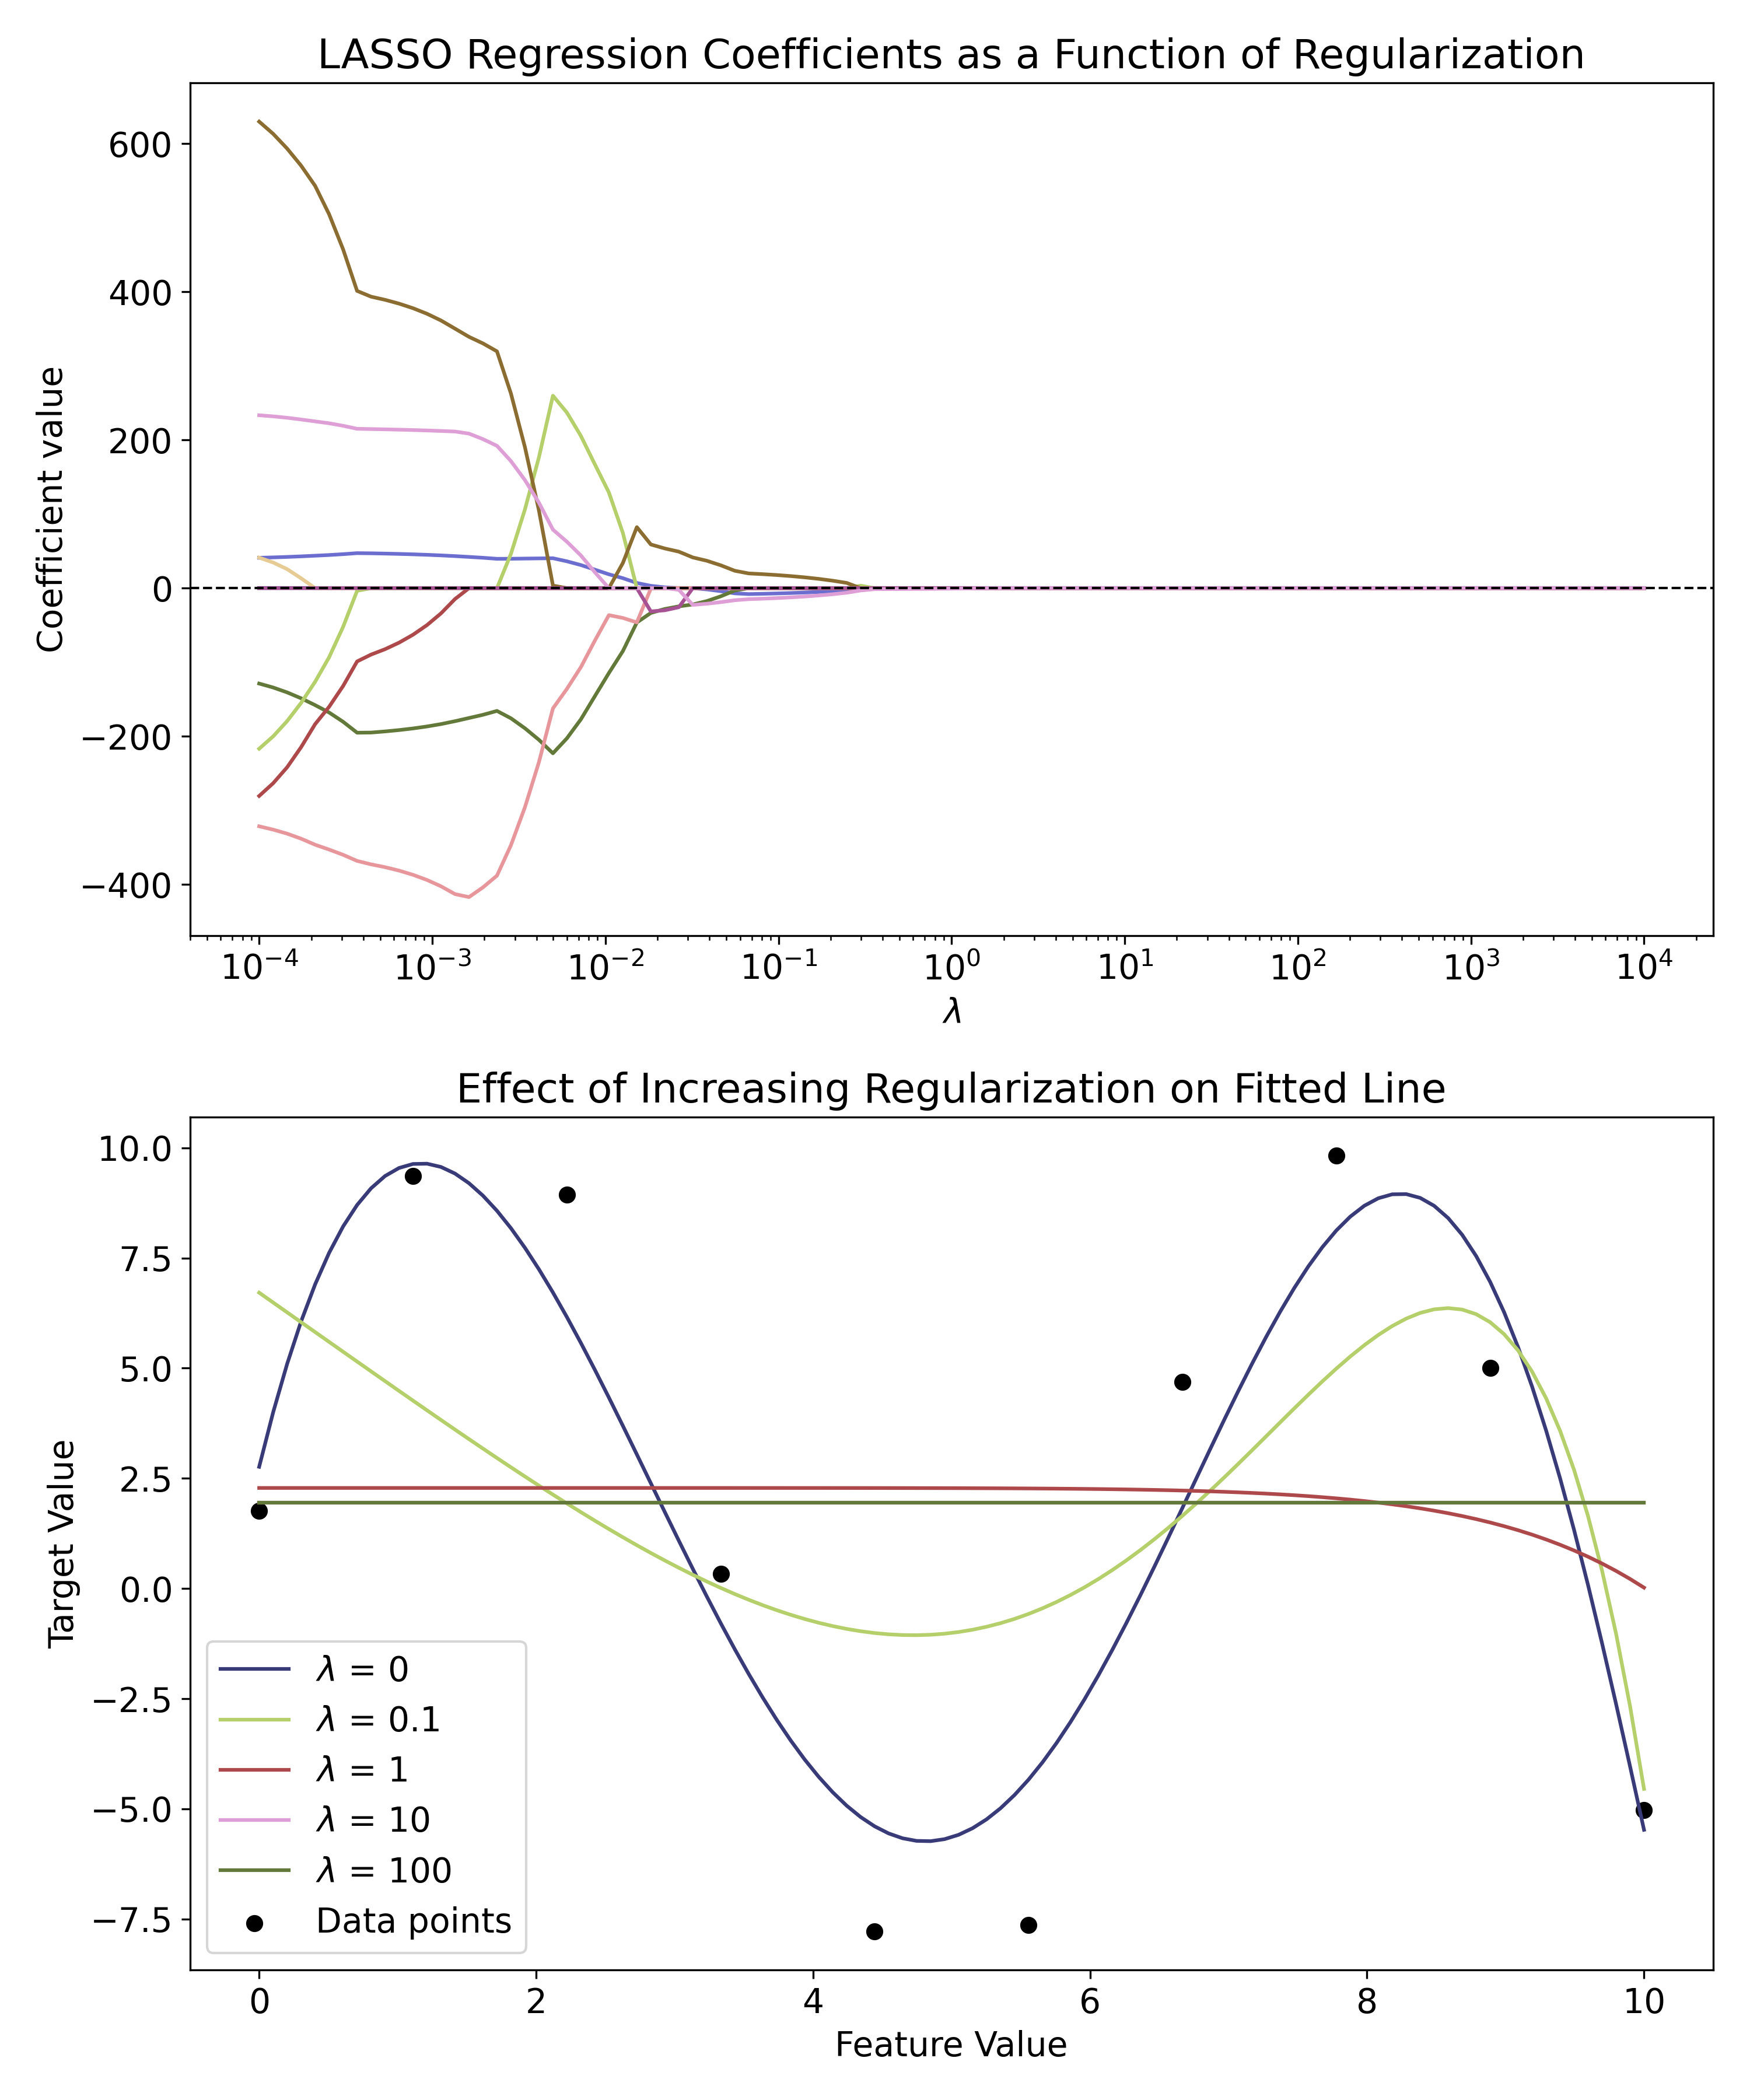
\includegraphics[width=1.0\linewidth]{img/lasso_lambda_effect}
		\caption{LASSO Regression Coefficients and the Effect of Regularization. \\ The \textbf{top plot} shows LASSO Regression coefficients as a function of the regularization parameter $\lambda$. Each line represents a different feature's coefficient, demonstrating how increasing $\lambda$ causes some coefficients to shrink to zero, effectively performing feature selection. The \textbf{bottom plot} illustrates the effect of $\lambda$ on the fitted non-linear model for 10 data points (synthetic data). As $\lambda$ increases, the model transitions from overfitting (high variance) to better generalization (low variance), as seen by the smoothing of the fitted lines.}
		\label{fig:lassolambdaeffect}
	\end{figure}
	
	\clearpage
	
	\subsection*{Random Forest}
	Random Forest is an ensemble learning method used for both classification and regression tasks. It operates by constructing multiple decision trees during training, and outputting the mode of the classes (classification) or mean prediction (regression) of the individual trees. We will first explore how decision trees are created and move on to understanding the Random Forest method. Note that only the classification case will be explained, as this is the focus of the current work.
	
	\subsubsection*{Decision Trees}
	A decision tree is a flowchart-like structure in which each internal node represents a feature, each branch represents a decision rule, and each leaf node represents an outcome. The path from the root to a leaf represents classification rules \cite{hastieElementsStatisticalLearning2009}. An example of a simple decision tree is shown in Figure \ref{fig:decisiontreevisualization}A; the Gini impurity value shown in the tree will be explained in the text below.
	
	\begin{figure}[h]
		\centering
		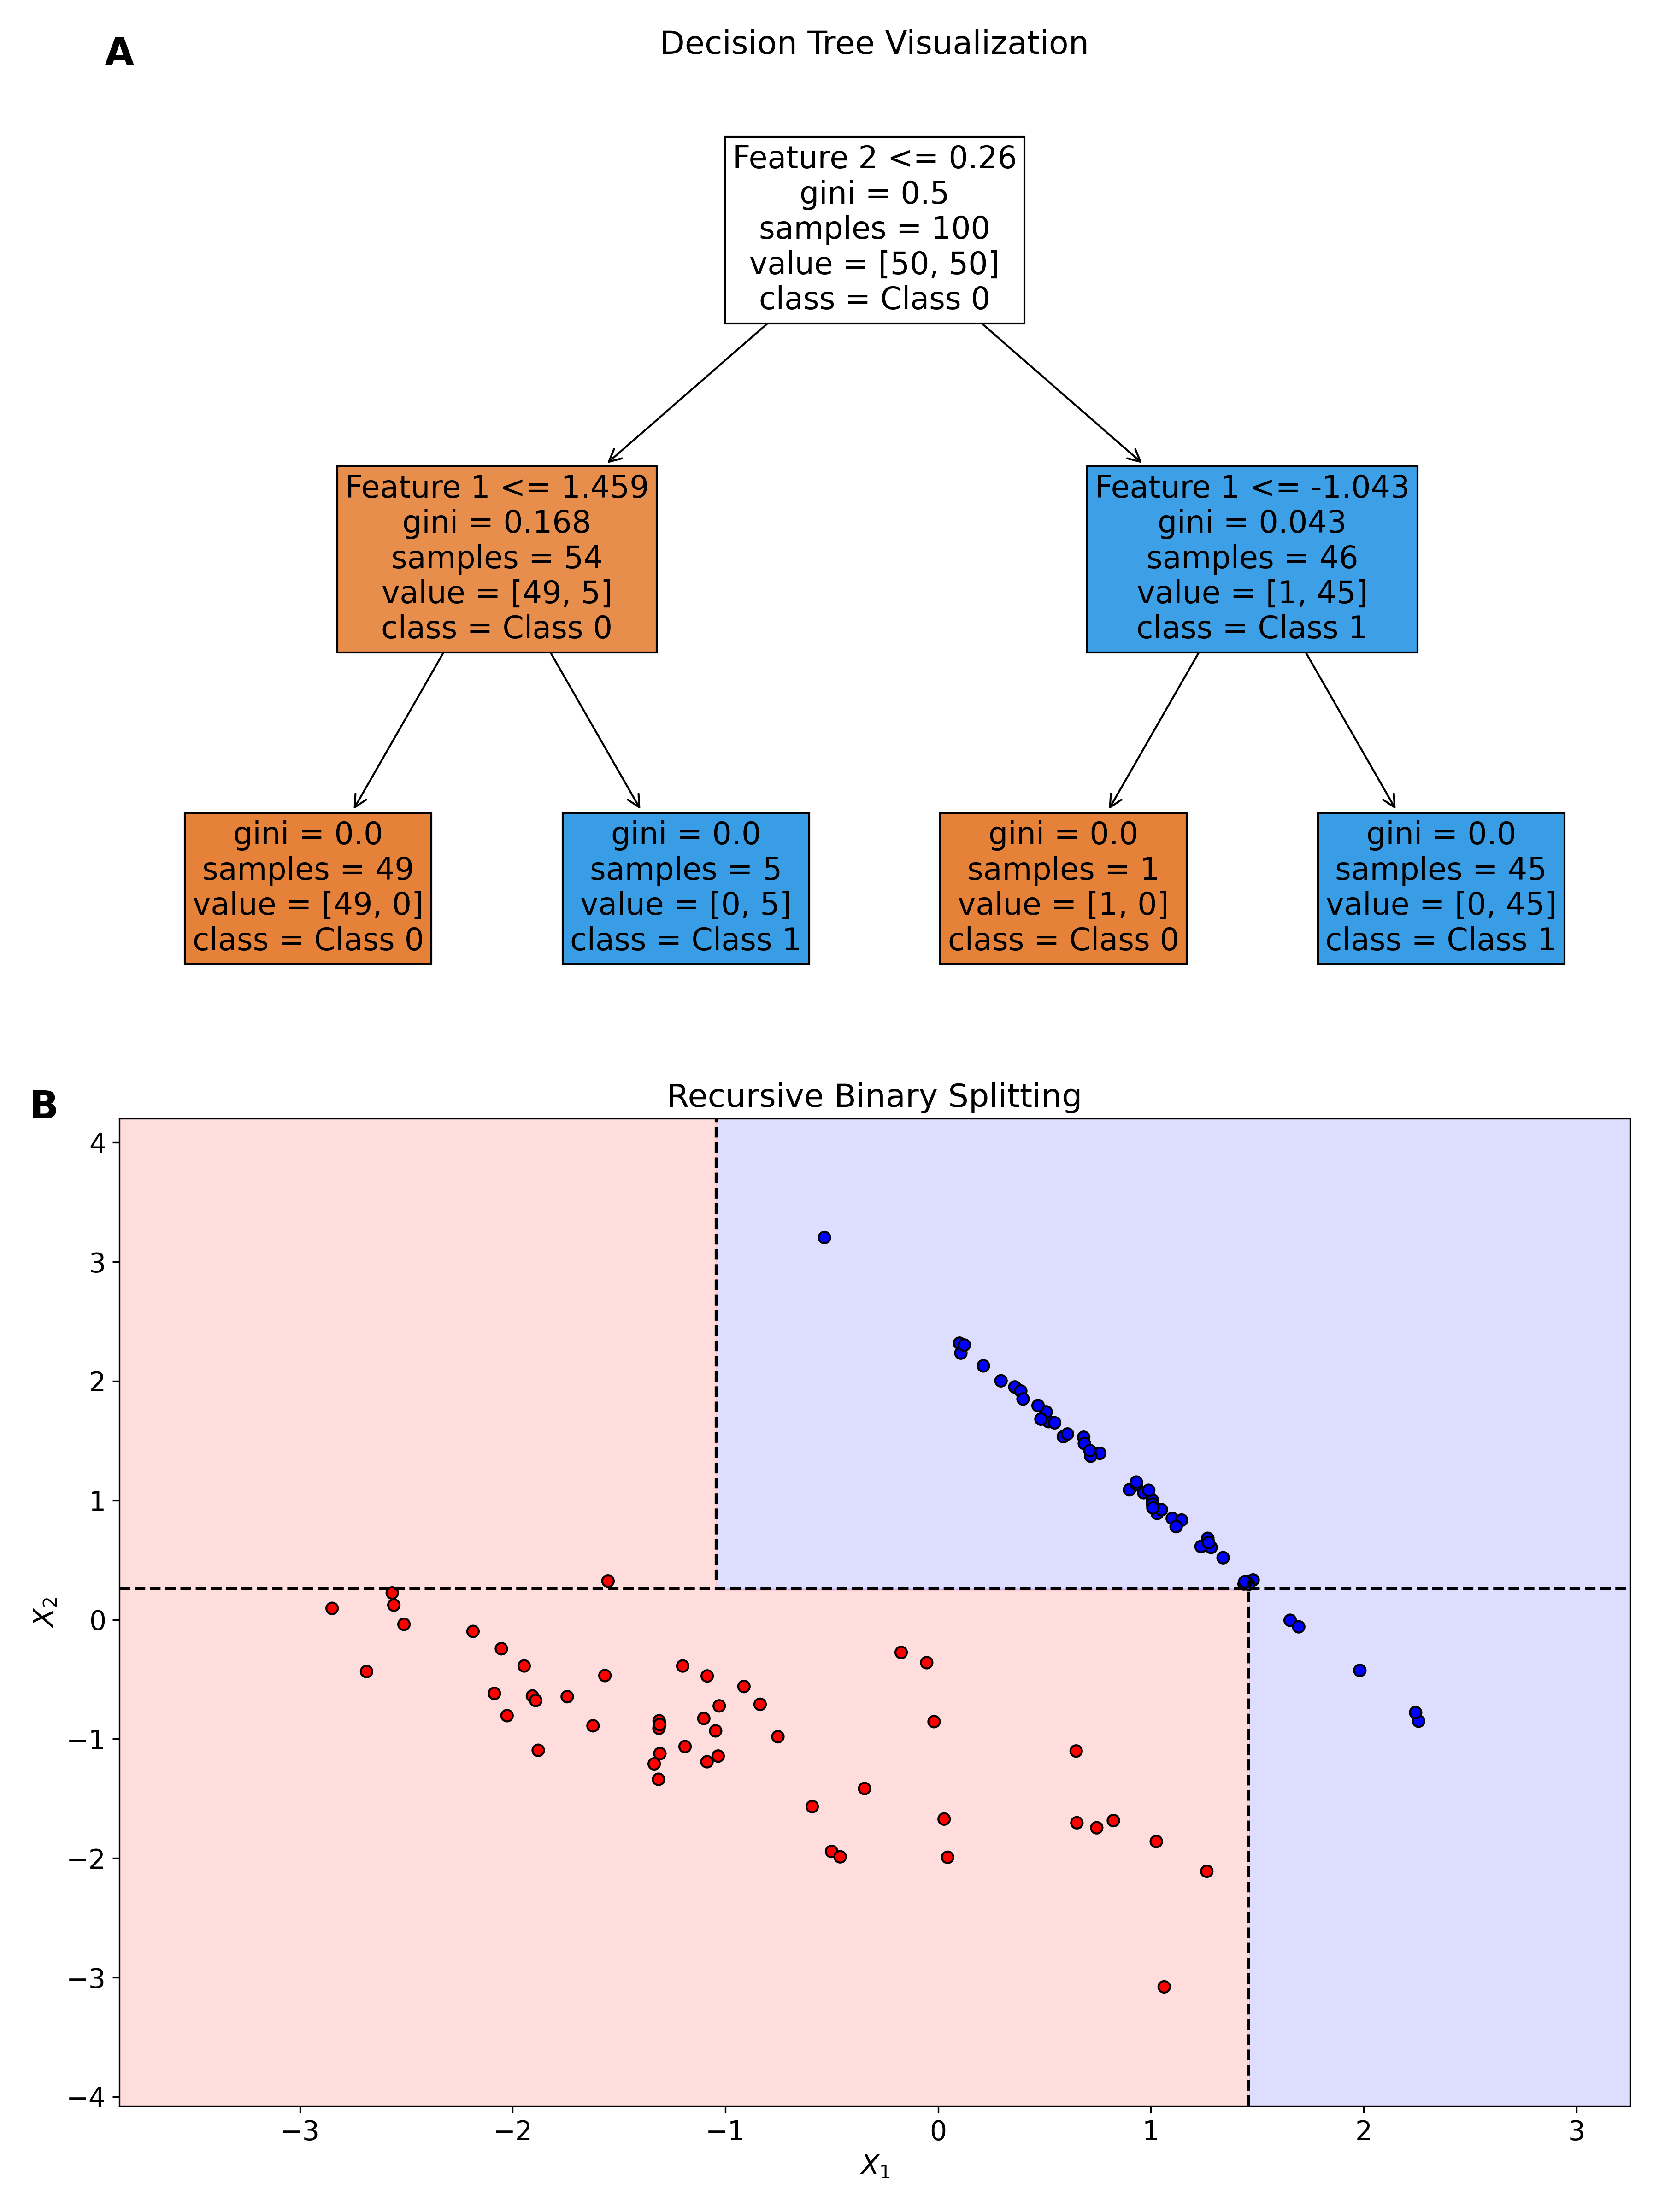
\includegraphics[width=1.0\linewidth]{img/decision_tree}
		\caption{Recursive Binary Splitting and Decision Tree Visualization. \\ This figure demonstrates the process of recursive binary splitting and the resulting decision tree on data that has two features: $X_1$ and $X_2$. The left plot (A) shows the decision boundaries created by a decision tree trained on a synthetic dataset, illustrating how the feature space is recursively split into regions, as indicated by the dashed lines. The right plot (B) visualizes the corresponding decision tree, with each internal node representing a decision rule based on feature thresholds, and leaf nodes representing class outcomes. Nodes are color-coded by the majority class, with class distributions and impurity measures (Gini index) displayed.}
		\label{fig:decisiontreevisualization}
	\end{figure}
	
	In constructing a decision tree, we aim to partition the feature space into regions where the response variable is as homogeneous as possible. This is done by recursively splitting the data based on certain criteria until a stopping condition is met.
	
	Given data that consists of \( p \) features and a response, for each of \( N \) observations \((x_i, y_i)\) for \( i = 1, 2, \ldots, N \), with \( x_i = (x_{i1}, x_{i2}, \ldots, x_{ip}) \), we model the response by partitioning the feature space into \( M \) regions \( R_1, R_2, \ldots, R_M \) and assigning class \( c_m \) to each region. The example in Figure \ref{fig:decisiontreevisualization} is split as follows:	
	\begin{enumerate}
		\item Feature 2 is split at \(X_2 = 0.26\) where the feature space at or below this point is assigned to class 0.
		\item Feature 1 is now split at \(X_1 = 1.459\).
		\item Finally, feature 1 is again split, now at \(X_1 = -1.043\).
	\end{enumerate}
	
	As visualized, this creates four regions in the feature space, which allows us to model the response as:
	\begin{equation*}
		\hat{f}(x) = \sum_{m=1}^{4} c_m I(x \in R_m)
	\end{equation*}
	where \( c_m \) is the class assigned to each region, and \( I(\cdots) \) is the indicator function, which is 1 if \( x \) is in region \( R_m \), and 0 otherwise. Since the data has only two classes, \( c_m \) will be either class 0 or class 1 for each region.
	
	But how do we decide where to split along each of the features? This is where we get into the splitting criterion, where there are two popular methods for classification tasks:
	
	\begin{itemize}
		\item \textbf{Gini impurity}:
		\begin{equation*}
			G = \sum_{i=1}^{C}p_i(1-p_i)
		\end{equation*}
		where $p_i$ is the probability of class $i$ in the node. This measures how often a randomly chosen element would be incorrectly classified.
		\item \textbf{Entropy}:
		\begin{equation*}
			H = -\sum_{i=1}^{C}p_i\log(p_i)
		\end{equation*}
		This measures the disorder or randomness of the data points in the node.
	\end{itemize}
	Since it is preferable to minimize both the Gini impurity and the entropy, the following step works for either criterion. Consider a feature \( j \) and a split point \( s \), and define the regions:
	\begin{equation*}
		R_1(j, s) = \{X|X_j \leq s\}\ \text{and}\ R_2(j, s) = \{X|X_j > s\}
	\end{equation*}
	
	The goal is then to find a \( j \) and \( s \) that minimize the function:
	\begin{equation*}
		\min_{j,s} \left[\frac{N_{R_1}}{N}C_{R_1} + \frac{N_{R_2}}{N}C_{R_2}\right]
	\end{equation*}
	where \( N_{R_1} \) and \( N_{R_2} \) are the number of samples in \( R_1 \) and \( R_2 \), and \( C_{R_1} \) and \( C_{R_2} \) is the splitting criterion value of these regions.
	
	After finding the best split, we now assign the class label for each region \( R_m \) as the majority class in that region:
	\begin{equation*}
		c_m = \arg \max_k \sum_{x_i \in R_m} I(y_i = k)
	\end{equation*}
	that is, the class label assigned for a given region is the class that appears most frequently within that region \cite{hastieElementsStatisticalLearning2009,sohilIntroductionStatisticalLearning2022}.
	
	Utilizing the functions mentioned so far for producing a decision tree could, however, lead to a problematic situation. One way to optimize the tree would be to grow it deep enough to assign each data point to its own node, resulting in an overly complex model. To prevent this, several methods can be employed:
	\begin{itemize}
		\item \textbf{Maximum depth}: Directly limit how deep the tree is allowed to grow.
		\item \textbf{Minimum samples per leaf}: Require a minimum number of samples in each leaf to avoid splits that result in nodes with very few data points.
		\item \textbf{Minimum samples per split}: Require a minimum number of samples to be present at a node before it can be split further.
		\item \textbf{Maximum leaf nodes}: Limit the number of leaf nodes in the tree to prevent excessive growth.
	\end{itemize}
	
	Once again, determining the optimal value for these hyperparameters is typically done through cross-validation.
	
	\subsubsection*{Random Forest}
	Building on the foundation of decision trees, Random Forest enhances the model's performance by combining multiple decision trees to form an ensemble. Each tree in the Random Forest is built using a bootstrap sample of the data, and at each split, a random subset of features is considered for splitting. The randomness helps in creating diverse trees that reduce the overall variance of the model.
	
	The Random Forest algorithm involves the following steps:
	\begin{enumerate}
		\item \textbf{Bootstrap sampling}: Randomly sample the dataset with replacement to create multiple bootstrap samples. Each tree is trained on a different bootstrap sample, introducing variability in the training data.
		\item \textbf{Tree construction}: For each bootstrap sample, grow a decision tree using a random subset of features at each split. This random selection of features further decorrelates the trees.
		\item \textbf{Aggregation}: Aggregate the predictions of all the trees to make the final prediction. For classification, the mode of the predicted classes is used.
	\end{enumerate}
	
	One might notice the aggressive attempt at decorrelating different trees in Random Forests. The reason for this is that if we can successfully create an ensemble of decorrelated trees, the variance of the model is reduced significantly more than if the trees are correlated. To understand this, consider \( n \) uncorrelated random variables \( X_1, X_2, \ldots, X_n \), each with the same variance \( \sigma^2 \). The variance of the sum of these variables is the sum of their variances \cite{moodIntroductionTheoryStatistics1973}. Mathematically:
	\begin{equation*}
		\text{Var}\left(\frac{1}{n} \sum_{i=1}^{n} X_i \right) = \frac{1}{n^2} \sum_{i=1}^{n} \text{Var}(X_i)
	\end{equation*}
	Simplifying:
	\begin{equation*}
		\frac{1}{n^2} \sum_{i=1}^{n} \text{Var}(X_i) = \frac{1}{n^2} \sum_{i=1}^{n} \sigma^2 = \frac{\sigma^2}{n}
	\end{equation*}
	Thus, the variance of the average of uncorrelated random variables decreases proportionally to \( \frac{1}{n} \).
	
	Now, if we instead consider \( n \) random variables \( X_1, X_2, \ldots, X_n \) that are highly correlated, let \( \rho \) represent the average correlation coefficient between any two variables.  For correlated variables, the covariance \( \text{Cov}(X_i, X_j) \) for \( i \neq j \) is \( \rho \sigma^2 \). 
	
	The variance now includes both the variance of the individual variables and the covariance between them:
	\begin{equation*}
		\text{Var}\left(\frac{1}{n}\sum_{i=1}^{n}X_i\right) = \frac{1}{n^2} \left(\sum_{i=1}^{n} \text{Var}(X_i) + \sum_{i \neq j} \text{Cov}(X_i, X_j)\right)
	\end{equation*}
	Given that \( \text{Var}(X_i) = \sigma^2 \) and \( \text{Cov}(X_i, X_j) = \rho \sigma^2 \), we can simplify further:
	\begin{align*}
		\frac{1}{n^2} \left(\sum_{i=1}^{n} \text{Var}(X_i) + \sum_{i \neq j} \text{Cov}(X_i, X_j)\right) &= \frac{1}{n^2}(n\sigma^2 + n(n-1)\rho\sigma^2) \\
		&= \frac{\sigma^2}{n} + \rho\sigma^2\left(1 - \frac{1}{n}\right)
	\end{align*}
	
	This shows that the variance reduction achieved through averaging is much less significant when the variables are correlated, as the additional term \( \rho\sigma^2\left(1 - \frac{1}{n}\right) \) does not decrease as rapidly with increasing \( n \). Hence, the effectiveness of Random Forests in reducing variance is due to the decorrelation of trees, leading to a more robust and generalizable model.
	
\section*{Methods}

\section*{Results}

\section*{Discussion}

\newpage
\printbibliography

\end{document}